\documentclass[tikz,border=2pt]{standalone}

\usepackage{amsmath}
\usepackage{pifont}  % for \ding symbols
\usepackage{xcolor}
\usepackage{tikz}
\usetikzlibrary{arrows.meta,positioning,fit,backgrounds,calc,decorations.pathreplacing,patterns,shapes.geometric}
\usepackage{pgfplots}
\pgfplotsset{compat=1.18}
\usepgfplotslibrary{groupplots,fillbetween}

% ── Color palette (NeurIPS-style, colorblind-friendly) ──
\definecolor{bestcolor}{HTML}{E8F5E9}
\definecolor{gaincolor}{HTML}{1B5E20}
\definecolor{cStandard}{HTML}{BF616A}   % muted red
\definecolor{cAOI}{HTML}{5E81AC}        % steel blue
\definecolor{cDelta}{HTML}{A3BE8C}      % sage green
\definecolor{cVisual}{HTML}{D08770}     % muted orange
\definecolor{cASR}{HTML}{B48EAD}        % muted purple
\definecolor{cNarr}{HTML}{88C0D0}       % light blue
\definecolor{cAccent}{HTML}{EBCB8B}     % warm yellow
\definecolor{cGray}{HTML}{4C566A}       % dark gray
\definecolor{cLightGray}{HTML}{D8DEE9}  % light gray

\begin{document}

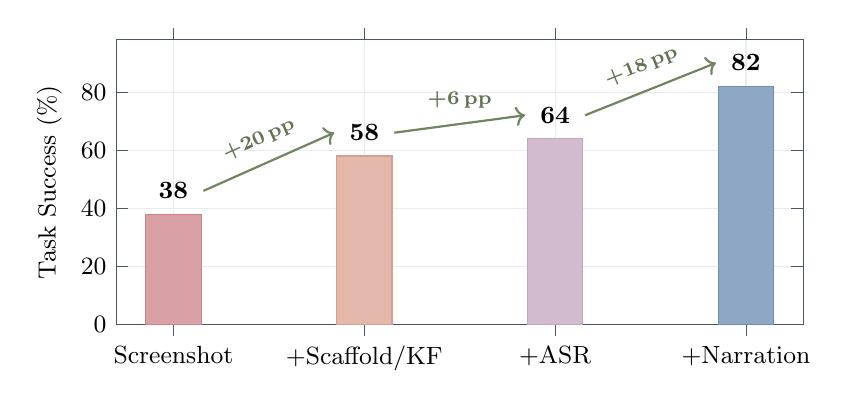
\begin{tikzpicture}
\begin{axis}[
    width=0.85\columnwidth,
    height=5.2cm,
    ybar,
    bar width=20pt,
    ymin=0, ymax=98,
    ylabel={Task Success (\%)},
    ylabel style={font=\small},
    symbolic x coords={Screenshot, {+Keyframes}, {+ASR}, {+Narration}},
    xtick={Screenshot, {+Keyframes}, {+ASR}, {+Narration}},
    xticklabels={Screenshot, {+Scaffold/KF}, +ASR, +Narration},
    xticklabel style={font=\small},
    ytick={0,20,40,60,80},
    yticklabel style={font=\small},
    grid=major,
    major grid style={cLightGray!60},
    axis line style={cGray},
    tick style={cGray},
    enlarge x limits=0.10,
    % nodes near coords,
    % nodes near coords style={font=\small\bfseries, /pgf/number format/fixed},
    % every node near coord/.append style={above=1pt},
]
\addplot[ybar, bar shift=0pt,fill=cStandard!60, draw=cStandard!80]
    coordinates {(Screenshot, 38)};
\addplot[ybar, bar shift=0pt,fill=cVisual!60, draw=cVisual!80]
    coordinates {({+Keyframes}, 58)};
\addplot[ybar, bar shift=0pt,fill=cASR!60, draw=cASR!80]
    coordinates {({+ASR}, 64)};
\addplot[ybar, bar shift=0pt,fill=cAOI!70, draw=cAOI!90]
    coordinates {({+Narration}, 82)};

% Named value labels above the bars
\node (v38) at (axis cs:Screenshot,38)
  [above=2pt, font=\small\bfseries] {38};

\node (v58) at (axis cs:{+Keyframes},58)
  [above=2pt, font=\small\bfseries] {58};

\node (v64) at (axis cs:{+ASR},64)
  [above=2pt, font=\small\bfseries] {64};

\node (v82) at (axis cs:{+Narration},82)
  [above=2pt, font=\small\bfseries] {82};

% Delta annotations inside the axis using axis cs
\draw[->, thick, cDelta!70!black]
  ([xshift=2pt]v38.east) -- ([xshift=-2pt]v58.west)
  node[midway, above=2pt, font=\scriptsize\bfseries, text=cDelta!60!black, sloped] {+20\,pp};
\draw[->, thick, cDelta!70!black]
  ([xshift=2pt]v58.east) -- ([xshift=-2pt]v64.west)
  node[midway, above=2pt, font=\scriptsize\bfseries, text=cDelta!60!black] {+6\,pp};
\draw[->, thick, cDelta!70!black]
  ([xshift=2pt]v64.east) -- ([xshift=-2pt]v82.west)
  node[midway, above=2pt, font=\scriptsize\bfseries, text=cDelta!60!black, sloped] {+18\,pp};
\end{axis}
\end{tikzpicture}

\end{document}